%%%%%%%%%%%%%%%%%%%%%%%%%%%%%%%%%%%%%%%%%
% Short Sectioned Assignment LaTeX Template Version 1.0 (5/5/12)
% This template has been downloaded from: http://www.LaTeXTemplates.com
% Original author:  Frits Wenneker (http://www.howtotex.com)
% License: CC BY-NC-SA 3.0 (http://creativecommons.org/licenses/by-nc-sa/3.0/)
%%%%%%%%%%%%%%%%%%%%%%%%%%%%%%%%%%%%%%%%%

%----------------------------------------------------------------------------------------
%	PACKAGES AND OTHER DOCUMENT CONFIGURATIONS
%----------------------------------------------------------------------------------------

\documentclass[paper=a4, fontsize=11pt]{scrartcl} % A4 paper and 11pt font size
% ---- Entrada y salida de texto -----

\usepackage[T1]{fontenc} % Use 8-bit encoding that has 256 glyphs
\usepackage[utf8]{inputenc}
%\usepackage[default]{sourcesanspro}
\usepackage{fourier} % Use the Adobe Utopia font for the document - comment this line to return to the LaTeX default
% ---- Idioma --------

\usepackage[spanish, es-tabla]{babel} % Selecciona el español para palabras introducidas automáticamente, p.ej. "septiembre" en la fecha y especifica que se use la palabra Tabla en vez de Cuadro

% ---- Code insertion ----
\usepackage{minted}
\usepackage[breakable]{tcolorbox} %Genera boxes, lo usamos para el codigo
\BeforeBeginEnvironment{minted}{\begin{tcolorbox}[breakable]}%
	\AfterEndEnvironment{minted}{\end{tcolorbox}}%
\BeforeBeginEnvironment{inputminted}{\begin{tcolorbox}[breakable]}%
	\AfterEndEnvironment{inputminted}{\end{tcolorbox}}%

\usepackage{xpatch} %permite abrir environments al ejecutar ciertos comandos

\xpretocmd{\inputminted}{\begin{tcolorbox}}{}{}%
	\xapptocmd{\inputminted}{\end{tcolorbox}}{}{}%

\setminted{
fontsize=\small,
breaklines,
breaksymbolleft=
}
% ---- Otros paquetes ----
\usepackage{dirtree}
\usepackage{vmargin}

\usepackage{url} % ,href} %para incluir URLs e hipervínculos dentro del texto (aunque hay que instalar href)
\usepackage{hyperref} % ,href} %para incluir URLs e hipervínculos dentro del texto (aunque hay que instalar href)
\hypersetup{
	colorlinks=true,
	linkcolor=blue,
	filecolor=magenta,      
	urlcolor=blue,
}

\usepackage{xcolor}
\definecolor{light-gray}{gray}{0.95}
\definecolor{alizarin}{rgb}{0.82, 0.1, 0.26}
\definecolor{nyellow}{rgb}{0.91, 0.656, 0.0}
%\definecolor{indigo}{rgb}{0.29, 0.0, 0.51}
%	\textcolor{red}{p}
%	\textcolor{orange}{r}
%	\textcolor{yellow}{a}
%	\textcolor{green}{c}
%	\textcolor{blue}{t}
%	\textcolor{indigo}{i}
%	\textcolor{violet}{c}
%	\textcolor{red}{a}
%	\textcolor{orange}{s}
%	\textcolor{yellow}{,}
%	\textcolor{green}{I}
%	\textcolor{blue}{S}
%	\textcolor{indigo}{E}

\usepackage{amsmath,amsfonts,amsthm} % Math packages
%\usepackage{graphics,graphicx, floatrow} %para incluir imágenes y notas en las imágenes
\usepackage{graphics,graphicx, float} %para incluir imágenes y colocarlas
\usepackage[export]{adjustbox}
\graphicspath{{imagenes/}}

% Para hacer tablas comlejas
%\usepackage{multirow}
%\usepackage{threeparttable}

%\usepackage{sectsty} % Allows customizing section commands
%\allsectionsfont{\centering \normalfont\scshape} % Make all sections centered, the default font and small caps

%Remove warnings
\usepackage{silence}
\WarningFilter{scrartcl}{Usage of package `fancyhdr'}

\usepackage{fancyhdr} % Custom headers and footers
\pagestyle{fancyplain} % Makes all pages in the document conform to the custom headers and footers
\fancyhead{} % No page header - if you want one, create it in the same way as the footers below
\fancyfoot[L]{} % Empty left footer
\fancyfoot[C]{} % Empty center footer
\fancyfoot[R]{\thepage} % Page numbering for right footer
\renewcommand{\headrulewidth}{0pt} % Remove header underlines
\renewcommand{\footrulewidth}{0pt} % Remove footer underlines
\setlength{\headheight}{13.6pt} % Customize the height of the header

\numberwithin{equation}{section} % Number equations within sections (i.e. 1.1, 1.2, 2.1, 2.2 instead of 1, 2, 3, 4)
\numberwithin{figure}{section} % Number figures within sections (i.e. 1.1, 1.2, 2.1, 2.2 instead of 1, 2, 3, 4)
\numberwithin{table}{section} % Number tables within sections (i.e. 1.1, 1.2, 2.1, 2.2 instead of 1, 2, 3, 4)

\setlength\parindent{0pt} % Removes all indentation from paragraphs - comment this line for an assignment with lots of text

\newcommand{\horrule}[1]{\rule{\linewidth}{#1}} % Create horizontal rule command with 1 argument of height

\setmarginsrb{2 cm}{1 cm}{2 cm}{2 cm}{1 cm}{1.5 cm}{1 cm}{1.5 cm} %Aumenta los márgenes

%----------------------------------------------------------------------------------------
%	TÍTULO Y DATOS DEL ALUMNO
%----------------------------------------------------------------------------------------

\title{Técnicas de los Sistemas Inteligentes\\ \quad\\
	Práctica 2: Problemas con restricciones en Minizinc  \hspace{0.05cm} }   

\author{Yeray López Ramírez	}                             

\renewcommand*\contentsname{hola}

\makeatletter
\let\thetitle\@title
\let\theauthor\@author
\let\thedate\@date
\makeatother

%----------------------------------------------------------------------------------------
% DOCUMENTO
%----------------------------------------------------------------------------------------

\begin{document}
\begin{titlepage}
	\centering
	%\textsc{\LARGE Universidad de Granada}\\[2.0 cm]    
	
\includegraphics[scale = 0.6]{ugr.png}\\[1.0 cm]
	\rule{\linewidth}{0.2 mm} \\[0.4 cm]
	{ \huge \bfseries \thetitle}\\
	\rule{\linewidth}{0.2 mm} \\[1.5 cm]
	
	\begin{minipage}{0.5\textwidth}
		\begin{flushleft} \large
			\theauthor 
			123456789-Z \\
			\href{mailto:fulanito@correo.ugr.es}{fulanito@correo.ugr.es}
		\end{flushleft}
	\end{minipage}~
	\begin{minipage}{0.5\textwidth}
		\begin{flushright} \large
			Curso: 2022-23 \\
			Grupo A, 15:30 - 17:30 (Martes)                   
		\end{flushright}
	\end{minipage}\\[1 cm]
	
	{\small \thedate}\\[1 cm]
	
	\vfill
	
\end{titlepage}


\newpage %inserta un salto de página
\newcommand{\code}[1]{\colorbox{light-gray}{\textcolor{red}{\texttt{#1}}}}
\newcommand{\high}[1]{\colorbox{light-gray}{\textcolor{yellow}{\texttt{#1}}}}
\newcommand{\highg}[1]{\colorbox{light-gray}{\textcolor{green}{\texttt{#1}}}}

\tableofcontents % para generar el índice de contenidos

\listoffigures

\listoftables

\newpage

%----------------------------------------------------------------------------------------
%	Cuestión 1
%----------------------------------------------------------------------------------------

\section*{Descripción de la práctica}

La práctica consiste en resolver 5 problemas con minizinc.

%----------------------------------------------------------------------------------------
%	Cuestión 2
%----------------------------------------------------------------------------------------

\section{Problema de la suma de conjuntos.}

\noindent\fbox{%
	\parbox{\textwidth}{\textbf{Enunciado:}
		Sea un conjunto de n números enteros $S = \{S_1, S_2, ... , S_n\}$. Se desea dividir este conjunto $S$ en
		dos subconjuntos disjuntos $S_1$ y $S_2$ (con $S_1 \cup S_2 = S, S_1 \cap S_2 = \emptyset$), de forma que la suma de los números en $S_1$ sea igual a la suma de los números en $S_2$.
	}%
}
\subsection{Realice la codificación del problema anterior y complete la tabla.}

% Please add the following required packages to your document preamble:
% \usepackage{graphicx}
% \usepackage[table,xcdraw]{xcolor}
% If you use beamer only pass "xcolor=table" option, i.e. \documentclass[xcolor=table]{beamer}
\begin{table}[H]
	\centering
	\caption{Resultados disjuntos}
	\label{tab:conjuntoa}
	\resizebox{0.7\textwidth}{!}{%
		\begin{tabular}{|c|c|c|c|}
			\hline
			\rowcolor[HTML]{EFEFEF} 
			Conjunto S                        & Conjunto S1 & Conjunto S2 & Suma de S1 y S2 \\ \hline
			\cellcolor[HTML]{FFFC9E}\{1,1,2\} & \{2\}       & \{1,1\}     & 2               \\ \hline
			\rowcolor[HTML]{FFCCC9} 
			\cellcolor[HTML]{FFFC9E}\{1,2,3,4,5,6,7,8\}   & UNSATISFIABLE & UNSATISFIABLE   & UNSATISFIABLE \\ \hline
			\cellcolor[HTML]{FFFC9E}\{1,1,2,4,4,5,6,7,8\} & \{4,7,8\}     & \{1,1,2,4,5,6\} & 19           \\ \hline
		\end{tabular}%
	}
\end{table}

Podemos observar que el segundo conjunto no es satisfactible ya que no existe ningún par de conjuntos que sumados den lo mismo. En el apartado c observé que la suma era 11 y 10 con $S_1=[5,6]$ y $S_2=[1,2,3,4]$.

\subsection{Añade una columna que indique el número total de soluciones.}

% Please add the following required packages to your document preamble:
% \usepackage{graphicx}
% \usepackage[table,xcdraw]{xcolor}
% If you use beamer only pass "xcolor=table" option, i.e. \documentclass[xcolor=table]{beamer}
\begin{table}[H]
	\centering
	\caption{Número soluciones disjuntos}
	\label{tab:conjuntob}
	\resizebox{0.9\textwidth}{!}{%
		\begin{tabular}{|c|c|c|c|c|}
			\hline
			\rowcolor[HTML]{EFEFEF} 
			Conjunto S &
			Conjunto S1 &
			Conjunto S2 &
			Suma de S1 y S2 &
			\multicolumn{1}{l|}{\cellcolor[HTML]{EFEFEF}Número soluciones} \\ \hline
			\cellcolor[HTML]{FFFC9E}\{1,1,2\}             & \{2\}     & \{1,1\}         & 2   & 2  \\ \hline
			\cellcolor[HTML]{FFFC9E}\{1,2,3,4,5,6,7,8\} &
			\cellcolor[HTML]{FFCCC9}UNSATISFIABLE &
			\cellcolor[HTML]{FFCCC9}UNSATISFIABLE &
			\cellcolor[HTML]{FFCCC9}UNSATISFIABLE &
			\cellcolor[HTML]{FFCCC9}0 \\ \hline
			\cellcolor[HTML]{FFFC9E}\{1,1,2,4,4,5,6,7,8\} & \{4,7,8\} & \{1,1,2,4,5,6\} & 19 & 14 \\ \hline
		\end{tabular}%
	}
\end{table}

El número de soluciones son SIMÉTRICAS. La mitad de ellas son permutaciones de S1 y S2 por lo que el número de soluciones reales sería 1,0,7.

\subsection{Modifique la codificación de forma que la diferencia entre la suma de S1 y S2 sea
	mínima.}

% Please add the following required packages to your document preamble:
% \usepackage{graphicx}
% \usepackage[table,xcdraw]{xcolor}
% If you use beamer only pass "xcolor=table" option, i.e. \documentclass[xcolor=table]{beamer}
\begin{table}[H]
	\centering
	\caption{Minimizar suma de conjuntos disjuntos}
	\label{tab:conjuntoc}
	\resizebox{\textwidth}{!}{%
		\begin{tabular}{|c|c|c|c|c|c|}
			\hline
			\rowcolor[HTML]{EFEFEF} 
			Conjunto S &
			S1 &
			S2 &
			\begin{tabular}[c]{@{}c@{}}Sum \\ S1\end{tabular} &
			\begin{tabular}[c]{@{}c@{}}Sum\\ S2\end{tabular} &
			Diff \\ \hline
			\cellcolor[HTML]{FFFC9E}\begin{tabular}[c]{@{}c@{}}\{99,14,82,47,82,50,77,45,23,92,\\ 52,90,46,57,29,25,74,25,30,70\}\end{tabular} &
			\{14 50 45 90 46 57 29 25 74 25 30 70\} &
			\{99 82 47 82 77 23 92 52\} &
			555 &
			554 &
			1 \\ \hline
			\cellcolor[HTML]{FFFC9E}\begin{tabular}[c]{@{}c@{}}\{35,82,97,30,38,78,18,39,35,93,49,\\ 47,30,57,43,21,92,51,89,80\}\end{tabular} &
			\cellcolor[HTML]{FFFFFF}\{35 35 49 57 43 21 92 51 89 80\} &
			\cellcolor[HTML]{FFFFFF}\{82 97 30 38 78 18 39 93 47 30\} &
			\cellcolor[HTML]{FFFFFF}552 &
			552 &
			0 \\ \hline
			\cellcolor[HTML]{FFFC9E}\begin{tabular}[c]{@{}c@{}}\{60,8,11,2,49,69,87,15,62,72,89,14,\\ 76,63,45,92,74,80,11,2\}\end{tabular} &
			\{8 11 15 14 76 63 45 92 74 80 11 2\} &
			\{60 2 49 69 87 62 72 89\} &
			491 &
			490 &
			1 \\ \hline
		\end{tabular}%
	}
\end{table}

\section{Problema de la regla}
\noindent\fbox{%
	\parbox{\textwidth}{\textbf{Enunciado:}
		Se tiene una regla de tamaño infinito a la que se desea realizar $m$ marcas en las posiciones
		(enteras) $x_1, x_2, \cdots ,x_m$ , de forma que las marcas están ordenadas en orden creciente: $x_1 < x_2< \cdots < x_m$ , de forma que la distancia entre cualquier par de marcas es distinta de todas las demás
		distancias, y de forma que la última marca $x_m$ es mínima. Por simplicidad, la primera marca se
		coloca en $x_1 = 0$. Codifique este problema y complete la tabla.
	}%
}

% Please add the following required packages to your document preamble:
% \usepackage{graphicx}
% \usepackage[table,xcdraw]{xcolor}
% If you use beamer only pass "xcolor=table" option, i.e. \documentclass[xcolor=table]{beamer}
\begin{table}[H]
	\centering
	\caption{Marcas con distancias diferentes}
	\label{tab:tabla2}
	\resizebox{0.8\textwidth}{!}{%
		\begin{tabular}{|
				>{\columncolor[HTML]{FFFC9E}}c |c|c|c|}
			\hline
			\cellcolor[HTML]{EFEFEF}\#marcas & \cellcolor[HTML]{EFEFEF}Posición de las marcas & \cellcolor[HTML]{EFEFEF}Última marca (Xm) & \cellcolor[HTML]{EFEFEF}Runtime \\ \hline
			3  & {[}0,1,3{]}                                       & 3  & 74msec     \\ \hline
			5  & {[}0, 2, 7, 8, 11{]}                              & 11 & 81msec     \\ \hline
			7  & {[}0, 2, 3, 10, 16, 21, 25{]}                     & 25 & 85msec     \\ \hline
			10 & {[}0, 1, 6, 10, 23, 26, 34, 41, 53, 55{]}         & 55 & 2s 622msec \\ \hline
			12 & {[}0, 2, 6, 24, 29, 40, 43, 55, 68, 75, 76, 85{]} & 85 & 4m 30s     \\ \hline
		\end{tabular}%
	}
\end{table}

A continuación, podemos observar cómo el número de marcas cambia en función del tamaño de \#marcas. Podemos notar que existe una tendencia más lineal en la posición de las marcas a medida que aumenta el tamaño de \#marcas. Por otro lado, el tiempo necesario para generar las marcas muestra un crecimiento exponencial, siendo especialmente lento cuando se alcanzan las 12 \#marcas.
\begin{figure}[H]
	\centering
	\begin{minipage}[b]{0.45\textwidth} % Primera figura
		\centering
		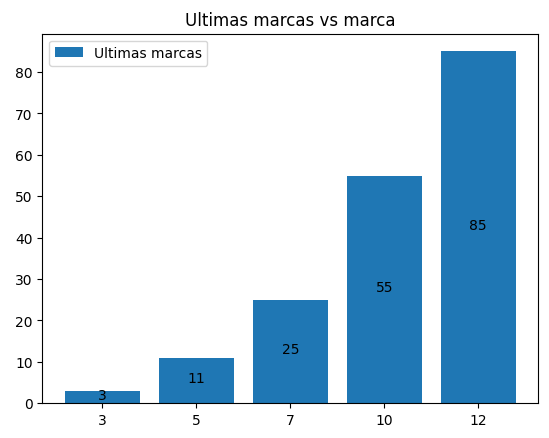
\includegraphics[scale=0.55]{marcasgrafica.png}
		\caption{Representación de la última marca en función del número de marcas}
		\label{fig:graficaRegla}
	\end{minipage}
	\hfill % Espacio horizontal entre las dos figuras
	\begin{minipage}[b]{0.45\textwidth} % Segunda figura
		\centering
		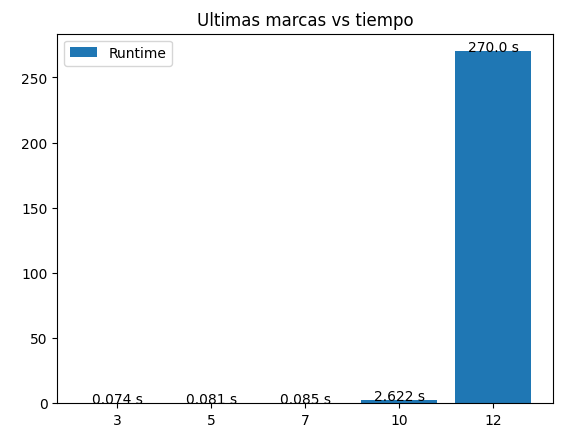
\includegraphics[scale=0.55]{marcasgrafica2.png}
		\caption{Representación de la última marca en función del tiempo}
		\label{fig:graficaRegla2}
	\end{minipage}
\end{figure}


\section{Problema de los horarios}
\noindent\fbox{%
	\parbox{\textwidth}{\textbf{Enunciado:}
		Se desea encontrar una asignación de horarios que satisfaga las siguientes condiciones:
		\begin{enumerate}
			\item  Existe un aula disponible en seis franjas consecutivas de 1h
			\item Existen nueve asignaturas (A1..A9)
			\item Las asignaturas {A1,A3,A4,A5,A8} deben impartirse en bloques de 2h consecutivas. El resto en bloques de 1h
			\item Cada día solo se puede impartir un bloque
			\item El profesor/a de cada asignatura es el siguiente: Prof1={A1,A3}; Prof2={A4,A5};
			Prof3={A6,A9}; Prof4={A2,A7,A8}.
			\item Cada profesor solo imparte un bloque al día excepto Prof4
			\item Varios profesores con restricciones horarias
			\item Varias asignaturas con restricciones diarias
		\end{enumerate}
		
		¿Cuál es el número de soluciones válidas obtenidas? ¿Existen soluciones simétricas? En caso de que la codificación propuesta contenga soluciones simétricas, ¿cómo se podrían evitar y cuál es el número de soluciones (no simétricas) obtenido? Explique cómo se consigue la rotura de simetrías (variables y/o restricciones utilizadas para ello), y entregue la solución MZN sin simetrías.
	}%
}
\quad \\ \quad \\
\[Sin \ terminar\]

\section{Problema de asignación de tareas}
\noindent\fbox{%
	\parbox{\textwidth}{\textbf{Enunciado:}
		Se pide encontrar una asignación de tiempos de inicio a las tareas de la tabla de forma que se pueda construir la casa en el menor tiempo posible. Cada tarea la realiza un único trabajador, pero los tres trabajadores pueden estar trabajando al mismo tiempo en tres tareas diferentes. 
	}%
}
% Please add the following required packages to your document preamble:
% \usepackage{graphicx}
% \usepackage[table,xcdraw]{xcolor}
% If you use beamer only pass "xcolor=table" option, i.e. \documentclass[xcolor=table]{beamer}
\begin{table}[H]
	\centering
	\caption{Tareas de construcción}
	\label{tab:tareas}
	\resizebox{0.6\textwidth}{!}{%
		\begin{tabular}{|l|l|l|l|}
			\hline
			\rowcolor[HTML]{000000} 
			{\color[HTML]{FFFFFF} \textbf{Tarea}} &
			{\color[HTML]{FFFFFF} \textbf{Descripción}} &
			{\color[HTML]{FFFFFF} \textbf{Duración}} &
			{\color[HTML]{FFFFFF} \textbf{Predecesoras}} \\ \hline
			A & Levantar muros & 5,7,10 & Ninguna \\ \hline
			B & Carpintería de trabajo  & 3,5,7  & A       \\ \hline
			C & Poner tejado            & 3,2,4  & B       \\ \hline
			D & Instalación eléctrica   & 2,5,8  & A       \\ \hline
			E & Pintado fachado         & 4,3,6  & C,D     \\ \hline
			F & Ventanas                & 3,2,1  & C,D,E   \\ \hline
			G & Jardín                  & 2,2,3  & C,D     \\ \hline
			H & Techado                 & 1,3,5  & A       \\ \hline
			I & Pintado interior        & 2,3,4  & F,H     \\ \hline
			J & Remates                 & 3,2,1  & G,I     \\ \hline
		\end{tabular}%
	}
\end{table}

\subsection{¿Cuál es la duración mínima de la construcción de la casa?}
Para la codificación del problema se ha utilizado una matriz de duraciones en función de la tarea(filas) y el trabajador(columnas). Cada Tarea tiene asociada un Inicio, un Fin y un Trabajador que la realiza. 
Tras aplicar todas las restricciones la duración mínima de construcción de la casa es de \textbf{17 días}. La última tarea en realizarse es la J (los remates).
% Please add the following required packages to your document preamble:
% \usepackage{graphicx}
% \usepackage[table,xcdraw]{xcolor}
% If you use beamer only pass "xcolor=table" option, i.e. \documentclass[xcolor=table]{beamer}
\begin{table}[H]
	\centering
	\caption{Construcción de la casa con 3 trabajadores}
	\label{tab:tabla4}
	\resizebox{0.6\textwidth}{!}{%
		\begin{tabular}{|c|c|c|c|c|c|c|c|c|c|c|}
			\hline
			\rowcolor[HTML]{EFEFEF} 
			\cellcolor[HTML]{656565}{\color[HTML]{FFFFFF} Tarea} & A & B & C  & D  & E  & F  & G  & H  & I  & J                                  \\ \hline
			\rowcolor[HTML]{FFFFFF} 
			\cellcolor[HTML]{FFFC9E}Inicio                       & 1 & 6 & 9  & 9  & 11 & 14 & 12 & 11 & 15 & {\color[HTML]{FE0000} \textbf{17}}          \\ \hline
			\rowcolor[HTML]{FFFFFF} 
			\cellcolor[HTML]{FFFC9E}Fin                          & 5 & 8 & 10 & 10 & 13 & 14 & 13 & 11 & 16 & {\color[HTML]{FE0000} \textbf{17}} \\ \hline
			\rowcolor[HTML]{FFCCC9} 
			\cellcolor[HTML]{FFFC9E}Trabajador & 1 & 1 & \cellcolor[HTML]{9AFF99}2 & 1 & \cellcolor[HTML]{9AFF99}2 & \cellcolor[HTML]{96FFFB}3 & 1 & 1 & 1 & \cellcolor[HTML]{96FFFB}3 \\ \hline
		\end{tabular}%
	}
\end{table}
% Please add the following required packages to your document preamble:
% \usepackage{graphicx}
% \usepackage[table,xcdraw]{xcolor}
% If you use beamer only pass "xcolor=table" option, i.e. \documentclass[xcolor=table]{beamer}
\begin{table}[H]
	\centering
	\caption{Diagrama de Gantt para 3 trabajadores}
	\label{tab:gant1}
	\resizebox{0.9\textwidth}{!}{%
		\begin{tabular}{|c|c|c|c|c|c|c|c|c|c|c|c|c|c|c|c|c|c|}
			\hline
			\cellcolor[HTML]{666666}{\color[HTML]{FFFFFF} Trabajadores} &
			1 &
			2 &
			3 &
			4 &
			5 &
			6 &
			7 &
			8 &
			9 &
			10 &
			11 &
			12 &
			13 &
			14 &
			15 &
			16 &
			17 \\ \hline
			tr1 &
			\cellcolor[HTML]{FFE599}A &
			\cellcolor[HTML]{FFE599}A &
			\cellcolor[HTML]{FFE599}A &
			\cellcolor[HTML]{FFE599}A &
			\cellcolor[HTML]{FFE599}A &
			\cellcolor[HTML]{F9CB9C}B &
			\cellcolor[HTML]{F9CB9C}B &
			\cellcolor[HTML]{F9CB9C}B &
			\cellcolor[HTML]{D0E0E3}D &
			\cellcolor[HTML]{D0E0E3}D &
			\cellcolor[HTML]{D9D2E9}H &
			\cellcolor[HTML]{EAD1DC}G &
			\cellcolor[HTML]{EAD1DC}G &
			\cellcolor[HTML]{FFFFFF} &
			\cellcolor[HTML]{E6B8AF}I &
			\cellcolor[HTML]{E6B8AF}I &
			\cellcolor[HTML]{FFFFFF} \\ \hline
			tr2 &
			\cellcolor[HTML]{FFFFFF} &
			\cellcolor[HTML]{FFFFFF} &
			\cellcolor[HTML]{FFFFFF} &
			\cellcolor[HTML]{FFFFFF} &
			\cellcolor[HTML]{FFFFFF} &
			\cellcolor[HTML]{FFFFFF} &
			\cellcolor[HTML]{FFFFFF} &
			\cellcolor[HTML]{FFFFFF} &
			\cellcolor[HTML]{E6B8AF}C &
			\cellcolor[HTML]{E6B8AF}C &
			\cellcolor[HTML]{D9EAD3}E &
			\cellcolor[HTML]{D9EAD3}E &
			\cellcolor[HTML]{D9EAD3}E &
			\cellcolor[HTML]{FFFFFF} &
			\cellcolor[HTML]{FFFFFF} &
			\cellcolor[HTML]{FFFFFF} &
			\cellcolor[HTML]{FFFFFF} \\ \hline
			tr3 &
			\cellcolor[HTML]{FFFFFF} &
			\cellcolor[HTML]{FFFFFF} &
			\cellcolor[HTML]{FFFFFF} &
			\cellcolor[HTML]{FFFFFF} &
			\cellcolor[HTML]{FFFFFF} &
			\cellcolor[HTML]{FFFFFF} &
			\cellcolor[HTML]{FFFFFF} &
			\cellcolor[HTML]{FFFFFF} &
			\cellcolor[HTML]{FFFFFF} &
			\cellcolor[HTML]{FFFFFF} &
			\cellcolor[HTML]{FFFFFF} &
			\cellcolor[HTML]{FFFFFF} &
			\cellcolor[HTML]{FFFFFF} &
			\cellcolor[HTML]{FFF2CC}F &
			\cellcolor[HTML]{FFFFFF} &
			\cellcolor[HTML]{FFFFFF} &
			\cellcolor[HTML]{FCE5CD}J \\ \hline
		\end{tabular}%
	}
\end{table}

\subsection{ ¿Qué tiempo tardarán, como mínimo, los cuatro trabajadores en finalizar la construcción?}
\noindent\fbox{%
	\parbox{\textwidth}{\textbf{Enunciado:}
		Se dispone de un cuarto trabajador, que podrá ser asignado para apoyar a cualquier tarea/trabajador con duración mayor o igual a 2 días, y consigue reducir la duración de esta tarea en un día.
	}%
}
\quad \\ \quad \\
Para la codificación del nuevo trabajador de apoyo se ha añadido un vector de bool donde cada posición representa la tarea y su valor False/True si el trabajador está en esa tarea o no. Las restricciones del trabajador de apoyo es igual que la del resto de trabajadores.
Tras aplicar los cambios del nuevo trabajador, la duración mínima de construcción de la casa es de \textbf{13 días}. La última tarea en realizarse es la J (los remates).

% Please add the following required packages to your document preamble:
% \usepackage{graphicx}
% \usepackage[table,xcdraw]{xcolor}
% If you use beamer only pass "xcolor=table" option, i.e. \documentclass[xcolor=table]{beamer}
\begin{table}[H]
	\centering
	\caption{Construcción de la casa con 3 trabajadores y 1 de apoyo}
	\label{tab:tabla4b}
	\resizebox{0.75\textwidth}{!}{%
		\begin{tabular}{|c|c|c|c|c|c|c|c|c|c|c|}
			\hline
			\rowcolor[HTML]{EFEFEF} 
			\cellcolor[HTML]{656565}{\color[HTML]{FFFFFF} Tarea} &
			A &
			B &
			C &
			D &
			E &
			F &
			G &
			H &
			I &
			J \\ \hline
			\rowcolor[HTML]{FFFFFF} 
			\cellcolor[HTML]{FFFC9E}Inicio &
			1 &
			5 &
			7 &
			7 &
			9 &
			11 &
			9 &
			8 &
			12 &
			{\color[HTML]{FE0000} \textbf{13}} \\ \hline
			\rowcolor[HTML]{FFFFFF} 
			\cellcolor[HTML]{FFFC9E}Fin &
			4 &
			6 &
			8 &
			9 &
			10 &
			11 &
			10 &
			8 &
			12 &
			{\color[HTML]{FE0000} \textbf{13}} \\ \hline
			\rowcolor[HTML]{FFCCC9} 
			\cellcolor[HTML]{FFFC9E}Trabajador &
			1 &
			1 &
			\cellcolor[HTML]{9AFF99}2 &
			1 &
			\cellcolor[HTML]{9AFF99}2 &
			\cellcolor[HTML]{96FFFB}3 &
			1 &
			1 &
			1 &
			\cellcolor[HTML]{96FFFB}3 \\ \hline
			\cellcolor[HTML]{FFFC9E}{\color[HTML]{000000} Apoyo} &
			{\color[HTML]{009901} True} &
			{\color[HTML]{009901} True} &
			{\color[HTML]{9A0000} False} &
			{\color[HTML]{009901} True} &
			{\color[HTML]{009901} True} &
			{\color[HTML]{9A0000} False} &
			{\color[HTML]{9A0000} False} &
			{\color[HTML]{009901} True} &
			{\color[HTML]{009901} True} &
			{\color[HTML]{9A0000} False} \\ \hline
		\end{tabular}%
	}
\end{table}
% Please add the following required packages to your document preamble:
% \usepackage{graphicx}
% \usepackage[table,xcdraw]{xcolor}
% If you use beamer only pass "xcolor=table" option, i.e. \documentclass[xcolor=table]{beamer}
\begin{table}[H]
	\centering
	\caption{Diagrama de Gantt para 3 trabajadores y 1 de apoyo}
	\label{tab:gant2}
	\resizebox{0.8\textwidth}{!}{%
		\begin{tabular}{|c|c|c|c|c|c|c|c|c|c|c|c|c|c|}
			\hline
			\cellcolor[HTML]{666666}{\color[HTML]{FFFFFF} Trabajadores} & 1     & 2     & 3     & 4     & 5     & 6     & 7     & 8     & 9     & 10    & 11 & 12    & 13    \\ \hline
			tr1 &
			\cellcolor[HTML]{FFE599}A &
			\cellcolor[HTML]{FFE599}A &
			\cellcolor[HTML]{FFE599}A &
			\cellcolor[HTML]{FFE599}A &
			\cellcolor[HTML]{F9CB9C}B &
			\cellcolor[HTML]{F9CB9C}B &
			\cellcolor[HTML]{D0E0E3}D &
			\cellcolor[HTML]{D0E0E3}D &
			\cellcolor[HTML]{D9D2E9}H &
			\cellcolor[HTML]{EAD1DC}G &
			\cellcolor[HTML]{EAD1DC}G &
			\cellcolor[HTML]{E6B8AF}I &
			\cellcolor[HTML]{FFFFFF} \\ \hline
			tr2 &
			\cellcolor[HTML]{FFFFFF} &
			\cellcolor[HTML]{FFFFFF} &
			\cellcolor[HTML]{FFFFFF} &
			\cellcolor[HTML]{FFFFFF} &
			\cellcolor[HTML]{FFFFFF} &
			\cellcolor[HTML]{FFFFFF} &
			\cellcolor[HTML]{E6B8AF}C &
			\cellcolor[HTML]{E6B8AF}C &
			\cellcolor[HTML]{D9EAD3}E &
			\cellcolor[HTML]{D9EAD3}E &
			\cellcolor[HTML]{FFFFFF} &
			\cellcolor[HTML]{FFFFFF} &
			\cellcolor[HTML]{FFFFFF} \\ \hline
			tr3 &
			\cellcolor[HTML]{FFFFFF} &
			\cellcolor[HTML]{FFFFFF} &
			\cellcolor[HTML]{FFFFFF} &
			\cellcolor[HTML]{FFFFFF} &
			\cellcolor[HTML]{FFFFFF} &
			\cellcolor[HTML]{FFFFFF} &
			\cellcolor[HTML]{FFFFFF} &
			\cellcolor[HTML]{FFFFFF} &
			\cellcolor[HTML]{FFFFFF} &
			\cellcolor[HTML]{FFFFFF} &
			\cellcolor[HTML]{FFF2CC}F &
			&
			\cellcolor[HTML]{FCE5CD}J \\ \hline
			trA                                                         & $T_A$ & $T_A$ & $T_A$ & $T_A$ & $T_B$ & $T_B$ & $T_D$ & $T_D$ & $T_E$ & $T_E$ &    & $T_I$ & \\ \hline
		\end{tabular}%
	}
\end{table}

\section{Problema sobre grafos}
\noindent\fbox{%
	\parbox{\textwidth}{\textbf{Enunciado:}
		Encontrar el conjunto mínimo de nodos de un grafo, de forma que para todo nodo, o bien éste pertenece a dicho conjunto, o bien alguno de sus vecinos pertenece al mismo. Implemente una codificación en MiniZinc para resolver este problema, y complete la tabla, generando 3 grafos aleatorios para cada tamaño de grafo (con tres semillas distintas).
	}%
}
% Please add the following required packages to your document preamble:
% \usepackage{graphicx}
% \usepackage[table,xcdraw]{xcolor}
% If you use beamer only pass "xcolor=table" option, i.e. \documentclass[xcolor=table]{beamer}
\begin{table}[H]
	\centering
	\caption{Conjunto mínimo con la media de 3 ejecuciones. Semillas 0,33,42}
	\label{tab:tablagrafos}
	\resizebox{0.8\textwidth}{!}{%
		\begin{tabular}{|c|l|l|}
			\hline
			\rowcolor[HTML]{EFEFEF} 
			Nº de nodos & \multicolumn{1}{c|}{\cellcolor[HTML]{EFEFEF}Mínimo número de nodos en el conjunto} & \multicolumn{1}{c|}{\cellcolor[HTML]{EFEFEF}Runtime (en milisegundos)} \\ \hline
			\rowcolor[HTML]{ECF4FF} 
			\cellcolor[HTML]{FFFC9E}10 & 2                                  & 165msec                   \\ \hline
			\rowcolor[HTML]{DAE8FC} 
			\cellcolor[HTML]{FFFC9E}20 & 3.33 (dos con 3 nodos y uno con 4) & 160msec                   \\ \hline
			\rowcolor[HTML]{ECF4FF} 
			\cellcolor[HTML]{FFFC9E}30 & 4,33 (dos con 4 nodos y uno con 5) & 175msec                   \\ \hline
			\rowcolor[HTML]{DAE8FC} 
			\cellcolor[HTML]{FFFC9E}40 & 6                                  & 385msec                   \\ \hline
			\rowcolor[HTML]{ECF4FF} 
			\cellcolor[HTML]{FFFC9E}50 & 8                                  & 10s 426msec (1 ejec a 2s) \\ \hline
			\rowcolor[HTML]{DAE8FC} 
			\cellcolor[HTML]{FFFC9E}60 & 9                                  & 2m 39s                    \\ \hline
		\end{tabular}%
	}
\end{table}

\begin{figure}[H] %con el [H] le obligamos a situar aquí la figura
	\centering
	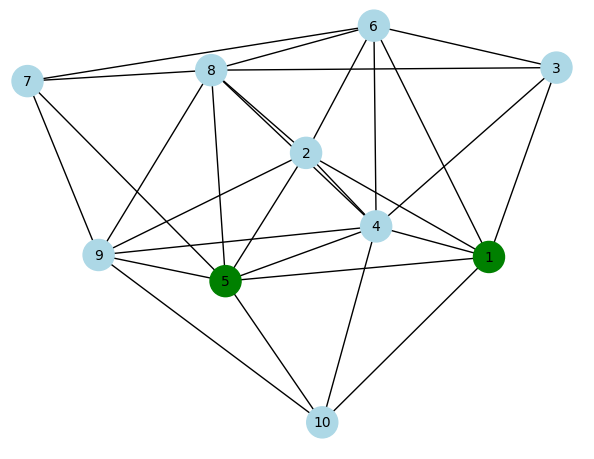
\includegraphics[scale=0.7]{grafo0.png}
	\caption{Representación del grafo con 10 nodos y semilla 0. Los nodos 1 y 5 son del conjunto mínimo}
	\label{fig:grafo}
\end{figure}

\subsection{¿Diría que este problema es escalable, es decir, se puede abordar su resolución en grafos de un tamaño considerable? Razone su respuesta.}
Observando los datos en la tabla, podemos ver que a medida que aumenta el número de nodos en el grafo, el número mínimo de nodos requeridos también aumenta, aunque no de manera lineal.\\


Por ejemplo, para el caso de 10 nodos, se requieren 2 nodos mínimos, mientras que para 20 nodos se requieren 3.33 nodos (aproximadamente 3 nodos). A pesar de que el número de nodos se ha duplicado, la cantidad mínima de nodos requeridos no se duplica de manera proporcional. Esto nos sugiere que el problema podría ser escalable, al menos en número de soluciones.\\


Sin embargo, a medida que el número de nodos aumenta el tiempo de ejecución aumenta exponencialmente, especialmente a partir de 40 nodos. De hecho, el tiempo de ejecución pasa de 10 segundos a más de 2 minutos para 50 y 60 nodos. Esto indica que el problema se vuelve más complejo y costoso computacionalmente a medida que se agregan más nodos, lo que hace que \code{NO} sea realmente \textbf{escalable en tiempo}.\\

\subsection{Bibliografía}
Toda la información obtenida ha sido de la documentación oficial de Minizinc \cite{minizinc} y de las diapositivas de clase \cite{mesejo}. Para dudas respecto a errores de codificación se ha recurrido a las páginas que todo el mundo bien conoce: stackoverflow \cite{stackoverflow} y chat \cite{chatgpt}.

\bibliography{citas} %archivo citas.bib que contiene las entradas 
\bibliographystyle{plain} % hay varias formas de citar

\end{document}
